\chapter{Quality of Service}

\section{Introduction}

\subsection{Traffic characteristics}

\paragraph{Voice}Voice traffic is predictable and smooth. However, voice is delay-sensitive and there is no reason to re-transmit voice if packets are lost. Therefore, voice packets must receive a higher priority than other types of traffic. Latency should be no more than \textbf{150 ms}. Jitter should be no more than \textbf{30 ms}, and voice packet loss should be no more than \textbf{1\%}. Voice traffic requires at least \textbf{30 Kbps} of bandwidth.

\paragraph{Video}Video traffic tends to be unpredictable, inconsistent, and bursty compared to voice traffic. Compared to voice, video is less resilient to loss and has a higher volume of data per packet. Latency should be no more than \textbf{400 ms}. Jitter should be no more than \textbf{50 ms}, and video packet loss should be no more than \textbf{1\%}. Video traffic requires at least \textbf{384 Kbps} of bandwidth.

\paragraph{Data}Data traffic is relatively insensitive to drops and delays compared to voice and video. The two main factors a network administrator needs to ask about the flow of data traffic are the following: Does the data come from an interactive application? Is the data mission critical?

\paragraph{Delay} Network congestion causes delay. Two types of delays are fixed and variable. A fixed delay is a specific amount of time a specific process takes, such as how long it takes to place a bit on the transmission media. A variable delay take an unspecified amount of time and is affected by factors such as how much traffic is being processed. \emph{Jitter} is the variation in the delay of received packets.

\subsection{QoS tools}

When the volume of traffic is greater than what can be transported across the network, network devices (router, switch, etc.) hold the packets in memory until resources become available to transmit them. If the number of packets continues to increase, the memory within the device fills up and packets are dropped. This problem can be solved by either increasing link capacity or implementing QoS.\\

A device implements QoS only when it is experiencing congestion. There are three categories of QoS tools: Classification and marking, Congestion avoidance, Congestion management. Refer to Figure \ref{QoStools} to help understand the sequence of how these tools are used when QoS is applied to packet flows.\\

\begin{figure}[hbtp]
\caption{QoS sequence}\label{QoStools}
\centering
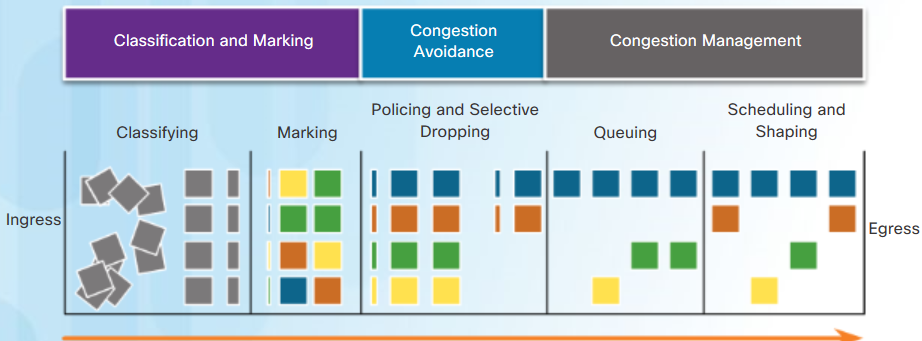
\includegraphics[ width=0.8\textwidth ]{pictures/QoStools.PNG}
\end{figure}

\section{Congestion management}
When traffic exceeds available network resources, Congestion management buffers and prioritizes packets before being transmitted to the destination. Common Cisco IOS-based congestion management tools include CBWFQ and LLQ algorithms.

\subsection{WFQ}

WFQ (Weighted Fair Queuing) is an automated scheduling method that provides fair bandwidth allocation to all network traffic. \\

WFQ applies priority to identified traffic and classifies it into flows, as shown in the figure \ref{WFQ}. WFQ then determines how much bandwidth each flow is allowed. WFQ classifies traffic into different flows based on packet header addressing.\\

\begin{figure}[hbtp]
\caption{WFQ example}\label{WFQ}
\centering
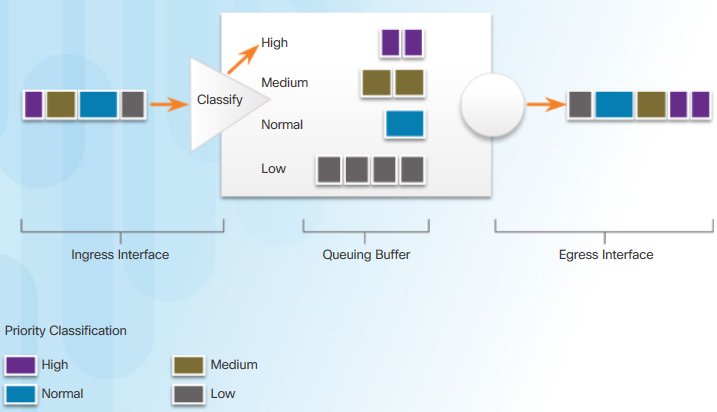
\includegraphics[ width=0.8\textwidth ]{pictures/WFQ.PNG}
\end{figure}

WFQ is not supported with tunneling and encryption. It does not allow users to take control over bandwidth allocation.

\subsection{CBWFQ}

Class-Based Weighted Fair Queuing (CBWFQ) extends the standard WFQ functionality to provide support for user-defined traffic classes. For CBWFQ, you define traffic classes based on match criteria including protocols, access control lists (ACLs), and input interfaces.\\

To characterize a class, you assign it bandwidth, weight, and queue limit. After a queue has reached its configured queue limit, adding more packets to the class causes tail drop. Tail drop means a router simply discards any packet that arrives at the end of a queue.

\subsection{LLQ}

The Low Latency Queuing (LLQ) feature brings strict priority queuing to CBWFQ. Strict PQ allows voice to be sent first. Without LLQ, CBWFQ services fairly based on weight; no class of packets may be granted strict priority. This scheme poses problems for voice traffic that is largely intolerant of delay.

\section{QoS models}
The three models for implementing QoS are: Best-effort model, Integrated services (IntServ), Differentiated services (DiffServ). Best-effort model means \emph{no QoS} is implemented. QoS is really implemented in a network using either IntServ or DiffServ.

\subsection{Best effort}

The best-effort model (meaning no QoS) treats all network packets in the same way. This model is used when QoS is not required. The table \ref{BestEffort} lists the benefits and drawbacks of the best effort model. 

\begin{table}[hbtp]
\centering
\caption{Pros and Cons of Best-effort}\label{BestEffort}
\begin{tabular}{ll}
\toprule
\head{Benefits} & \head{Drawbacks} \\ 
\midrule 
Most scalable & No guarantees of delivery \\  
Scalability is limited by bandwidth & Packets can arrive in any order \\ 
No special QoS mechanism required & No packets have preferential treatment \\ 
Easy to deploy & Critical data is treated the same as casual one \\ 
\bottomrule
\end{tabular}
\end{table} 

\subsection{Integrated services}

Integrated Services (IntServ) is a multiple-service model that can accommodate multiple QoS requirements.\\

It uses resource reservation and admission-control mechanisms as building blocks to establish and maintain QoS. Each individual communication must explicitly specify its traffic descriptor and requested resources to the network (Figure \ref{IntServ}). The edge router performs admission control to ensure that available resources are sufficient in the network.\\

\begin{figure}[hbtp]
\caption{Simple IntServ example}\label{IntServ}
\centering
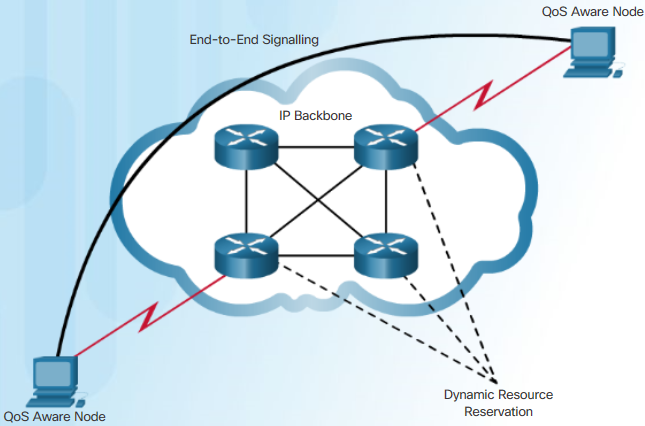
\includegraphics[scale=0.7]{pictures/IntServ.PNG}
\end{figure}

IntServ uses the \textbf{RSVP} (Resource Reservation Protocol) to reserve bandwidth for an application's traffic (e.g. VoIP) across the entire path. If this requested reservation fails along the path, the originating application does not send any data.\\

\begin{table}[hbtp]
\centering
\caption{Pros and Cons of IntServ}
\begin{tabular}{ll}
\toprule
\head{Benefits} & \head{Drawbacks} \\ 
\midrule 
Explicit end-to-end resource admission control & Resource intensive \\  
Per-request policy admission control & Not scalable \\ 
Signaling of dynamic port numbers &  \\ 
\bottomrule
\end{tabular}
\end{table} 

\subsection{Differentiated services}

The DiffServ design overcomes the limitations of both the best-effort and IntServ models. Unlike IntServ, DiffServ is not an end-to-end QoS strategy and does not use signaling. Instead, DiffServ uses a “soft QoS” approach (Figure \ref{DiffServ1}). For example, DiffServ can provide low-latency guaranteed service to voice or video while providing best-effort traffic to web traffic or file transfers.\\

\begin{figure}[hbtp]
\caption{Simple DiffServ example}\label{DiffServ1}
\centering
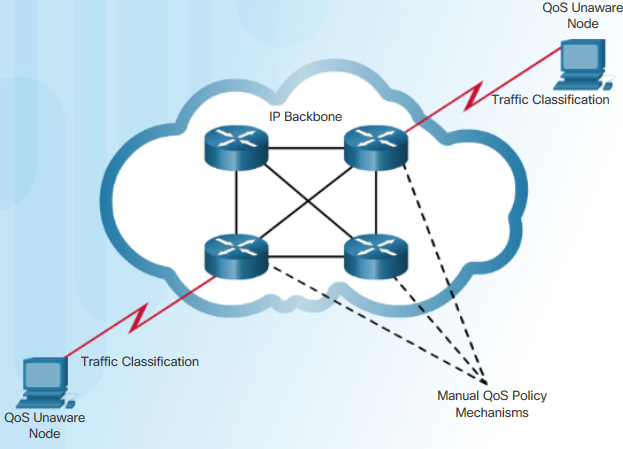
\includegraphics[scale=0.7]{pictures/DiffServ.PNG}
\end{figure}


Specifically, DiffServ divides network traffic into classes based on business requirements. Each of the classes can then be assigned a different level of service. You pay for a level of service. Throughout the network, the level of service you paid for is recognized and your package is given either preferential or normal traffic, depending on what you requested.\\

\begin{table}[hbtp]
\centering
\caption{Pros and Cons of DiffServ}\label{DiffServ2}
\begin{tabular}{ll}
\toprule
\head{Benefits} & \head{Drawbacks} \\ 
\midrule 
Highly scalable & No absolute guarantee of delivery \\  
Many different levels of quality & Requires complex mechanisms \\ 
\bottomrule
\end{tabular}
\end{table} 

\section{Classification and marking}

Before a packet can have a QoS policy applied to it, the packet has to be classified. Classification and marking identifies types of packets. Traffic should be classified and marked as close to its source as technically and administratively feasible. This defines the trust boundary. \\

Marking means that we are adding a value to the packet header. Devices receiving the packet look at this field to see if it matches a defined policy.\\

Trusted endpoints have the capabilities and intelligence to mark application traffic to the appropriate Layer 2 CoS and/or Layer 3 DSCP values. Examples of trusted endpoints include IP phones, wireless access points, videoconferencing gateways and systems, IP conferencing stations, and more.\\

Methods of classifying traffic flows at Layer 2 and 3 include using interfaces, ACLs, and class maps.

\subsection{Marking at Layer 2}

802.1Q is the IEEE standard that supports VLAN tagging at layer 2 on Ethernet networks. The 802.1Q standard also includes the QoS prioritization scheme known as IEEE 802.1p. The 802.1p standard uses the first three bits in the Tag Control Information (TCI) field (Figure \ref{CoS}). Known as the Priority (PRI) field, this 3-bit field identifies the Class of Service (CoS) markings.\\

\begin{figure}[hbtp]
\caption{Ethernet Class of Service values}\label{CoS}
\centering
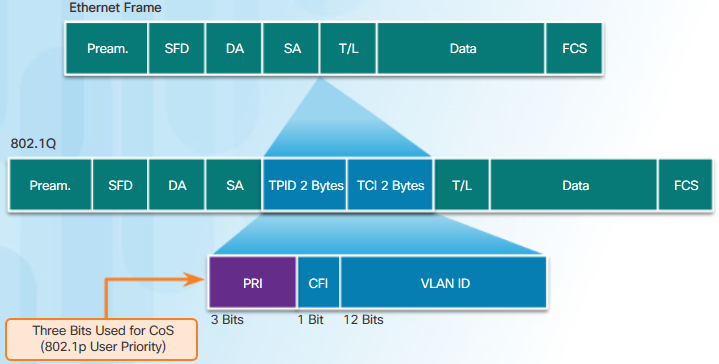
\includegraphics[ width=0.8\textwidth ]{pictures/CoS.PNG}
\end{figure}

\subsection{Marking at Layer 3}

The benefit of deploying Layer 3 marking is that it can carry QoS information end-to-end unlike Layer 2 marking, which changes frame header as well as QoS information hop by hop.\\

Both IPv4 and IPv6 support an 8-bit field for marking, the Type of Service (ToS) field for IPv4 and the Traffic Class field for IPv6. Figure \ref{ToS} displays the contents of the 8-bit field. The field has 6-bits allocated for QoS, called the \textbf{DiffServ} Code Point (DSCP) field. The remaining two IP Extended Congestion Notification (ECN) bits can be used by ECN-aware routers to mark packets instead of dropping them. The ECN marking informs downstream routers that there is congestion in the packet flow. \\

\begin{figure}[hbtp]
\caption{Type of Service/Traffic Class Field}\label{ToS}
\centering
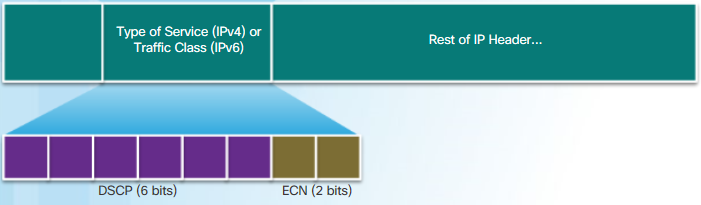
\includegraphics[ width=0.8\textwidth ]{pictures/ToS.PNG}
\end{figure}

The DSCP values are organized into three categories: 
\begin{itemize}
\item \textbf{Best-Effort (BE):} When a router experiences congestion, these packets will be dropped. No QoS plan is implemented.
\item \textbf{Expedited Forwarding (EF):} DSCP decimal value is 46 (binary 101110). At Layer 3, Cisco recommends that EF only be used to mark voice packets.
\item \textbf{Assured Forwarding (AF):} Use the 5 most significant DSCP bits to indicate queues and drop preference. As shown in Figure \ref{DSCP}, the first 3 most significant bits are used to designate the class. The 4th and 5th most significant bits are used to designate the drop preference. The 6th most significant bit is set to zero. The AFxy formula shows how the AF values are calculated. For example, AF32 belongs to class 3 (binary 011) and has a medium drop preference (binary 10).
\end{itemize}

\begin{figure}[hbtp]
\caption{Assured forwarding values}\label{DSCP}
\centering
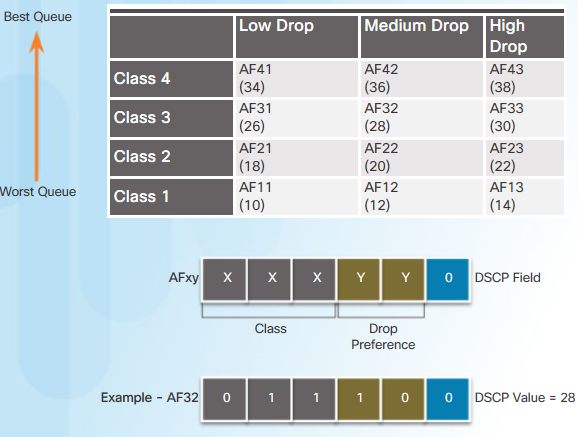
\includegraphics[ scale=0.7 ]{pictures/DSCP.PNG}
\end{figure}

\section{Congestion Avoidance}

We avoid congestion by dropping lower-priority packets before congestion occurs. When the queue fills up to the maximum threshold, a small percentage of packets are dropped. When the maximum threshold is passed, all packets are dropped. WRED, traffic shaping, and traffic policing are three mechanisms provided by Cisco IOS QoS software to prevent congestion. 

\paragraph{WRED} is the primary congestion avoidance tool. It regulates TCP data traffic before tail drops (caused by queue overflows) occur.

\paragraph{Traffic shaping}retains excess packets in a queue and then schedules the excess for later transmission over increments of time. The result of traffic shaping is a smoothed packet output rate, as shown in Figure \ref{Spacing}. Ensure that you have sufficient memory when enabling shaping.\\

\begin{figure}[hbtp]
\caption{Spacing traffic example}\label{Spacing}
\centering
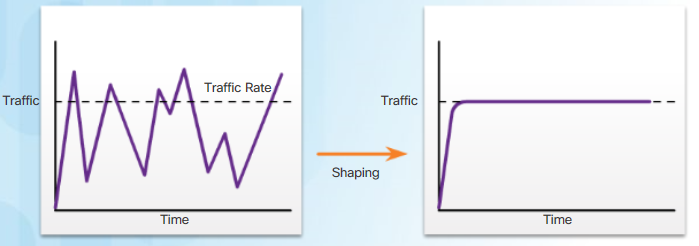
\includegraphics[scale=0.7]{pictures/Spacing.PNG}
\end{figure}

\paragraph{Traffic policing}Shaping is an outbound concept; packets going out an interface get queued and can be shaped. In contrast, policing is applied to inbound traffic on an interface. When the traffic rate reaches the configured maximum rate, excess traffic is dropped (or remarked), as shown in figure \ref{policing}.\\

\begin{figure}[hbtp]
\caption{Spacing traffic example}\label{policing}
\centering
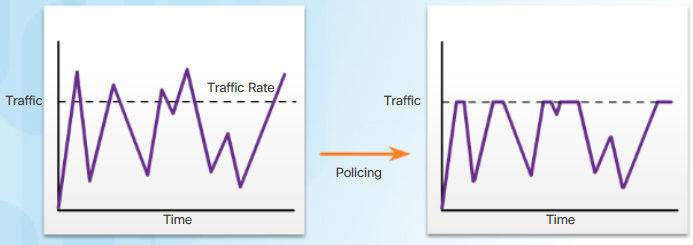
\includegraphics[ scale=0.7 ]{pictures/policing.PNG}
\end{figure}